%%%%%%%%%%%%%%%%%%%%%%%%%%%%%%%%%%%%%%%%%%%%%%%%%%%%%%%%%%%%%%%%%%%%%%
%%                     Transition
%%%%%%%%%%%%%%%%%%%%%%%%%%%%%%%%%%%%%%%%%%%%%%%%%%%%%%%%%%%%%%%%%%%%%%
%\color{blue}
\subsection{Glyph: \glyph{Transition}}\label{sec:transition}

A transition is a process transforming a set of states or entities in another set of states or entities.

\begin{glyphDescription}
 \item[SBO]\mbox{}\\ SBO:0000167 ! reaction
 \item[origin]\mbox{}\\ One or several \glyph{consumption} arcs (section \ref{sec:consumption}) or one or several \glyph{production} arcs (section~\ref{sec:production}).
 \item[target]\mbox{}\\ One or several \glyph{production} arcs (section \ref{sec:production}).
 \item[node]\mbox{}\\ A transition is represented by a square box. The arcs linking it to the state/entity nodes are attached to the center of opposite sides. The modulatory arcs point to the other two sides. A \glyph{transition} connected to \glyph{production} arcs on opposite sides is a reversible transition.
 \end{glyphDescription}

\begin{figure}[H]
  \centering
  \includegraphics[scale = 0.5]{images/transition}
  \caption{The \PD glyph for \glyph{transition}.}
  \label{fig:transition}
\end{figure}

A transition is the basic process node in SBGN. It describes a process that transforms a given set of biochemical entities --- macromolecules, simple 
chemicals or unspecified entities --- into another set of biochemical entities. Such a transformation might imply modification of covalent bonds (conversion), 
modification of the relative position of constituents (conformational transition) or movement from one compartment to another (translocation).

A cardinality label may be associated with \glyph{consumption} (section \ref{sec:consumption}) or 
\glyph{production} (section \ref{sec:production}) arc indicating the stoichiometry of a process. This is required to eliminate ambiguity when the exact composition of the number of copies of the inputs or outputs to a reaction are ambiguous from the diagram. 

The following example illustrates the use of a \glyph{transition} node to 
represent the phosphorylation of a protein in a state transition diagram.

\begin{center}
\scalebox{0.3}{\includegraphics{examples/transition-phosphorylation}}
\end{center}

The following example illustrates the use of a \glyph{transition} node to represent an reaction between two reactants that generates three products. 

\begin{center}
\scalebox{0.3}{\includegraphics{examples/transition-reaction}}
\end{center}

The following example illustrates the use of a \glyph{transition} node to represent a translocation. The large round-cornered rectangle represents a compartment border (see section \ref{sec:compartment}).

\begin{center}
\scalebox{0.3}{\includegraphics{examples/transition-translocation}}
\end{center}

The following example illustrates the use of a \glyph{transition} node to represent the reversible opening and closing of an ionic channel in a state transition diagram.

\begin{center}
\scalebox{0.3}{\includegraphics{examples/transition-reversible}}
\end{center}

When such a reversible process is assymetrically modulated, it should be represented by two different processes in State Transition. The following example illustrates the use of two \glyph{transition} nodes to represent the reversible activation of a G-protein coupled receptor. In the absence of any effector, an equilibrium exists between the inactive and active forms. The agonist stabilises the active form, while the inverse agonist stabilises the inactive form.

\begin{center}
\scalebox{0.3}{\includegraphics{examples/transition-modulated}}
\end{center}

The following example presents the conversion of two galactoses into a lactose. Galactoses are represented by only one \glyph{simple chemical}, the cardinality being carried by the \glyph{consumption} arc.

\begin{center}
\scalebox{0.3}{\includegraphics{examples/transition-dimerisation}}
\end{center}

\normalcolor
